\lab{Python}{Optimization with Scipy}{scipy.optimize}
\label{lab:Optimization1}
\objective{Introduce some of the basic optimization functions available in \li{scipy.optimize}}

The Optimize package in Scipy has several types of optimizing algorithms.
This lab will introduce some of the basic types of algorithms included.

You can learn about all of the functions at \url{http://docs.scipy.org/doc/scipy/reference/optimize.html}.

First we will test out a few of the optimization algorithms on the Rosenbrock Function, which satisfies the equation $f(x,y) = (1-x)^2 + 100(y-x^2)^2$.
The Rosenbrock fuction is a common optimization algorithm checking function, so it is included in the optimize package, as well as its jacobian(\li{rosen_der} \emph{I think}) and its hessian.

\begin{figure}
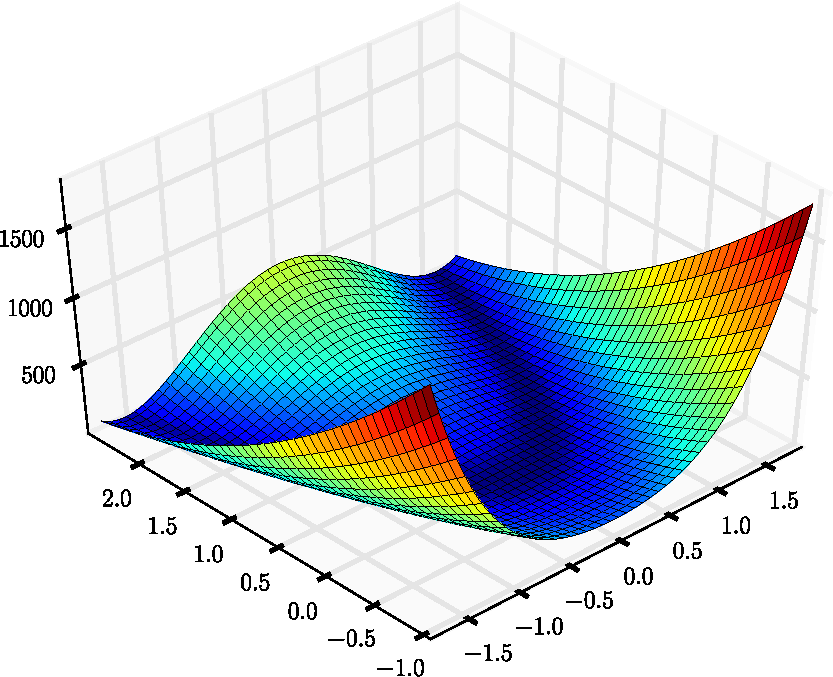
\includegraphics[width=\textwidth]{Rosenbrock.pdf}
\caption{$f(x,y) = (1-x)^2 + 100(y-x^2)^2$}
\label{opt:rosenbrock}
\end{figure}

We will use the \li{scipy.optimize.minimize} function and test each of its algorithms (under "method" on the online documentation page for \li{minimize}). Note that there are also several functions such as \li{fmin} and \li{fmin_powell}. These are equivalent to functions accsessed with the \li{minimize} function.

Note that for some algorithms, you'll need the gradient and/or hessian.
You may recognize some of these algorithms, and several of them will be discussed in greater detail later. For this lab, you do not need to understand how they work.

\begin{problem}

Import the \li{scipy.optimize} module as \li{opt}. Now use the \li{opt.minimize} function to find the minimimum of the Rossenbrock function, found as \li{opt.rosen}. Test each of the algorithms. Part of the output of \li{opt.minimize} is the number of iterations each algorithm took. Which finds the minimum the fastest? Do any of the algorithms fail to find the (correct) minimum of the Rossenbrock?
Make sure to start with the same initial guess in all of them. As an example we'll minimize the Rossenbrock with the Nelder-Mead method.

\begin{lstlisting}
x0 = np.array([1.3, 0.7, 0.8, 1.9, 1.2])
opt.minimize(opt.rosen, x0, method='nelder-mead', options={'xtol': 1e-8, 'disp': True})
\end{lstlisting}

\emph{Extra: How would you maximize the Rossenbrock function?}
\end{problem}

When are optimizing functions, it is easiest when we are dealing with convex functions, as they only have one global minimum. However, this is frequently not the case, and sometimes we need pick the global minimum out of many local minima.

For example, consider the function
%This is the crazy function that I came up with to stump the algorithms
\[
z = r^2 (1+ 2sin(4r)^2)
\]
Where
\[
r = \sqrt{(x-4)^2 + y^2}
\]
Essentially this is a wavey crater offset from the origin by 1 along the $x$ axis.
\begin{figure}%sorry, this is a really bad picture using mathmatica. Python was being difficult graphing it
\includegraphics[width=\textwidth]{MultiMin.pdf}
\caption{$z = r^2 (1+ 2sin(4r)^2)$}
\label{opt:muiltmin}
\end{figure}
This function has many local minima which we will see proves difficult for the minimization algorithms.

For example, if we use the \li{opt.fmin} function (which employs the Neader-Mead method, otherwise known as the downhill simplex method) the algorithm fails to find the global maximum, and instead comes to rest on a local maximum.
\begin{lstlisting}
def multimin(x):
    r = np.sqrt((x[0]+1)**2 + x[1]**2)
    return r**2 *(1+ np.sin(4*r)**2)

x0 = [-2,-2]
res = opt.fmin(multimin, x0, xtol=1e-8, disp=True)
print res
print multimin(res)
print multimin([-1,0])
\end{lstlisting}
Output
\begin{lstlisting}
Optimization terminated successfully.
         Current function value: 5.488169
         Iterations: 56
         Function evaluations: 134
[-2.03513929 -2.08611595]
5.48816865696
0.0
\end{lstlisting}

However, scipy does have some tools to help us with these problems. Specifically, we can use the \li{opt.basinhopping} function. 
Conceptually, most of the minimizing algorithms use to derivitive the function to search for the downhill direction of the function and make guesses downhill. Often they overshoot the minimum and come back. You can think of it as a ball rolling down a hill that slowly loses momentum as is overshoots the valleys and goes up the hill sides. Eventually the ball comes to rest at the bottom of a valley - hopefully the lowest valley. However, if there are many valleys (or loval minima) the ball can get stuck in one that's not the lowest valley.
The \li{opt.basinhopping} algorithim uses the same minimizing functions (in fact, you can tell it whatever minimizing algorithm you can pass to \li{opt.minimize}). However, once it settles on a minimum, the basinhopping algorithm pops it out of the this minimum (depending on how we set the "hopping" distance)  and hopefully out of the minimum its stuck it. If the new minimum it finds is even smaller than the last, it starts over with the new minimum.

\emph{Only Scipy Version 0.12+ has \li{opt.basinhopping}, in earlier versions, such as 0.11 you won't find it}
%I've seen a real cool animation of this -feasible to do in python?
\begin{problem}

Look at the documentation for the \li{opt.basinhopping} function online and use it to find the global minimum of our function with the same \li{x0}. Use the same \li{Nelder-Mead} algorithim with the same \li{xtol}. You will need to pass into the \li{opt.basinhopping} function a dictionary within a dictionary for the arguments of the minimizing algorithm to get all these options in.
Try it first with \li{stepsize=0.5} and then with \li{setsize=0.2}. Why doesn't it find the minimum the second time?

\end{problem}

%we still have curve fitting
%least squares programming -- but it seems that it's already been done in Volume One
Scipy also has functions to do curve fitting.

\begin{problem}
Use the \li{opt.curve_fit} function to fit a heating curve to 
\end{problem}


%minimizing scalar functions

%root finding


